\chapter{Finding Closest Pair of Points}

\parinf

\textbf{{Problem}:}  Given a set of points find the closest pair of points  in $\bbR^2$. 

\textbf{Input:} Set $S=\{(x_i,y_i)\mid x_i,y_i\in\bbR, \ \forall\ i\in[n]\}$. We denote $P_i=(x_i,y_i)$. 

\textbf{Output:} $P_i,P_j$ that are at minimum $l_2$ distance i.e. minimize $\sqrt{(x_i-x_j)^2+(y_i-y_j)^2}$. 

\section{Naive Algorithm}

Now the naive algorithm for this will be checking all pairs of points and take their distance and output the minimum one. There are total $\binom{n }{2}$ possible choices of pairs of points. And calculating the distance of each pair takes $O(1)$ time. So it will take $O(n^2)$ times to find the closest pair of points. \parinf

\textbf{Idea:} $\forall\ P_i,P_j\in S$ find distance $d(P_i,P_j)$ and return the minimum. Time taken is $O(n^2)$. 

\section{Divide and Conquer Algorithm}
\dfn[divide-n-Conquer]{Divide and Conquer}{
\begin{itemize}
\item Divide: Divide the problem into two parts (roughly equal)
\item Conquer: Solve each part individually recursively.  If the subproblem sizes are small enough, however, just solve the subproblems in a straightforward manner.
\item Combine: Combine  the solutions to the subproblems into the solution.
\end{itemize}
    }

\subsection{Divide}  So to divide the problem into two roughly equal parts we need to divide the points into two equal sets. That we can do by sorting the points by their $x-$coordinate. Suppose $S^x$ denote we get the new sorted array or points. And similarly we obtain $S^y$ which denotes the array of points after sorting $S$ by their $y-$coordinate.
\begin{center}
    \begin{minipage}{0.6\textwidth}
        \begin{algorithm}[H]
            \DontPrintSemicolon
            \SetKwProg{Fn}{Function}{:}{}
            \Fn{Divide}{
                Sort $S$ by $x-$coordinate and $y-$coordinate\;
                $S^x\longleftarrow S$ sorted by $x-$coordinate\;
                $S^y\longleftarrow S$ sorted by $y-$coordinate\;
                $\bar{x}\longleftarrow \lfloor \frac{n}{2}\rfloor $ highest $x-$coordinate\;
                $\bar{y}\longleftarrow \lfloor \frac{n}{2}\rfloor $ highest $y-$coordinate\;
                $S^L\longleftarrow \{P_i\mid x_i<\bar{x},\ \forall\ i\in[n]\}$\;
                $S^R\longleftarrow \{P_i\mid x_i\geq\bar{x},\ \forall\ i\in[n]\}$
            }
            \caption{Step 1 (Divide)}
        \end{algorithm}
        
    \end{minipage}
    \hspace{5mm}
    \begin{minipage}{0.35\textwidth}

\tikzset{every picture/.style={line width=0.75pt}} %set default line width to 0.75pt        

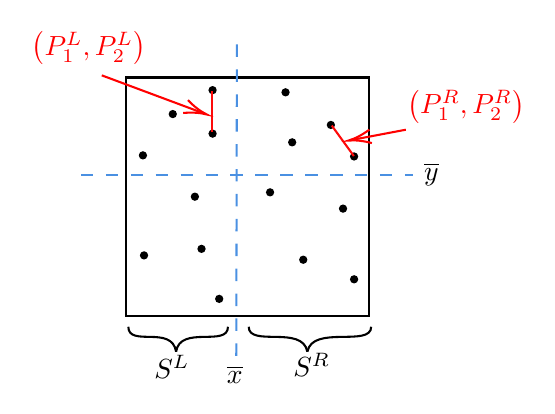
\begin{tikzpicture}[x=0.75pt,y=0.75pt,yscale=-1,xscale=1]
%uncomment if require: \path (0,325); %set diagram left start at 0, and has height of 325

%Shape: Rectangle [id:dp6499204868826074] 
\draw   (80.93,157.92) -- (198.12,157.92) -- (198.12,272.62) -- (80.93,272.62) -- cycle ;
%Straight Lines [id:da837478004805259] 
\draw [color={rgb, 255:red, 74; green, 144; blue, 226 }  ,draw opacity=1 ] [dash pattern={on 4.5pt off 4.5pt}]  (59.2,204.85) -- (219,204.85) ;
%Straight Lines [id:da7194776025159269] 
\draw [color={rgb, 255:red, 74; green, 144; blue, 226 }  ,draw opacity=1 ] [dash pattern={on 4.5pt off 4.5pt}]  (134.31,142) -- (134,295) ;
%Shape: Free Drawing [id:dp8916770831600931] 
\draw  [line width=3] [line join = round][line cap = round] (103.41,175.52) .. controls (103.41,175.52) and (103.41,175.52) .. (103.41,175.52) ;
%Shape: Free Drawing [id:dp7205705113694219] 
\draw  [line width=3] [line join = round][line cap = round] (179.58,180.76) .. controls (179.58,180.76) and (179.58,180.76) .. (179.58,180.76) ;
%Shape: Free Drawing [id:dp5723003936317532] 
\draw  [line width=3] [line join = round][line cap = round] (166.27,245.7) .. controls (166.27,245.7) and (166.27,245.7) .. (166.27,245.7) ;
%Shape: Free Drawing [id:dp19778776200558257] 
\draw  [line width=3] [line join = round][line cap = round] (89.56,243.61) .. controls (89.56,243.61) and (89.56,243.61) .. (89.56,243.61) ;
%Shape: Free Drawing [id:dp22218199289458562] 
\draw  [line width=3] [line join = round][line cap = round] (150.29,213.23) .. controls (150.29,213.23) and (150.29,213.23) .. (150.29,213.23) ;
%Shape: Free Drawing [id:dp9270216931653172] 
\draw  [line width=3] [line join = round][line cap = round] (157.74,165.04) .. controls (157.74,165.04) and (157.74,165.04) .. (157.74,165.04) ;
%Shape: Free Drawing [id:dp30577755696643694] 
\draw  [line width=3] [line join = round][line cap = round] (89.03,195.42) .. controls (89.03,195.42) and (89.03,195.42) .. (89.03,195.42) ;
%Shape: Free Drawing [id:dp8352617777328899] 
\draw  [line width=3] [line join = round][line cap = round] (125.78,264.56) .. controls (125.78,264.56) and (125.78,264.56) .. (125.78,264.56) ;
%Shape: Free Drawing [id:dp007121195742592068] 
\draw  [line width=3] [line join = round][line cap = round] (190.77,255.13) .. controls (190.77,255.13) and (190.77,255.13) .. (190.77,255.13) ;
%Shape: Free Drawing [id:dp9787419741468635] 
\draw  [line width=3] [line join = round][line cap = round] (160.94,189.14) .. controls (160.94,189.14) and (160.94,189.14) .. (160.94,189.14) ;
%Shape: Free Drawing [id:dp05782734388952204] 
\draw  [line width=3] [line join = round][line cap = round] (114.06,215.32) .. controls (114.06,215.32) and (114.06,215.32) .. (114.06,215.32) ;
%Shape: Free Drawing [id:dp020809307556031387] 
\draw  [line width=3] [line join = round][line cap = round] (122.59,184.95) .. controls (122.59,184.95) and (122.59,184.95) .. (122.59,184.95) ;
%Shape: Free Drawing [id:dp9236450749534464] 
\draw  [line width=3] [line join = round][line cap = round] (117.26,240.46) .. controls (117.26,240.46) and (117.26,240.46) .. (117.26,240.46) ;
%Shape: Free Drawing [id:dp9814876804759312] 
\draw  [line width=3] [line join = round][line cap = round] (185.44,221.08) .. controls (185.44,221.08) and (185.44,221.08) .. (185.44,221.08) ;
%Shape: Free Drawing [id:dp32677091280799897] 
\draw  [line width=3] [line join = round][line cap = round] (190.77,195.95) .. controls (190.77,195.95) and (190.77,195.95) .. (190.77,195.95) ;
%Shape: Free Drawing [id:dp7375869135394859] 
\draw  [line width=3] [line join = round][line cap = round] (122.59,164) .. controls (122.59,164) and (122.59,164) .. (122.59,164) ;
%Straight Lines [id:da2008032684012] 
\draw [color={rgb, 255:red, 253; green, 10; blue, 10 }  ,draw opacity=1 ]   (122.48,164.63) -- (122.48,184) ;
%Straight Lines [id:da715666979908854] 
\draw [color={rgb, 255:red, 253; green, 10; blue, 10 }  ,draw opacity=1 ]   (180.01,181.07) -- (190.66,195.74) ;
%Straight Lines [id:da6970165255401948] 
\draw [color={rgb, 255:red, 255; green, 0; blue, 0 }  ,draw opacity=1 ]   (215.7,183.06) -- (189.96,187.93) ;
\draw [shift={(188,188.3)}, rotate = 349.29] [color={rgb, 255:red, 255; green, 0; blue, 0 }  ,draw opacity=1 ][line width=0.75]    (10.93,-3.29) .. controls (6.95,-1.4) and (3.31,-0.3) .. (0,0) .. controls (3.31,0.3) and (6.95,1.4) .. (10.93,3.29)   ;
%Straight Lines [id:da5840245566165858] 
\draw [color={rgb, 255:red, 255; green, 0; blue, 0 }  ,draw opacity=1 ]   (69.21,156.87) -- (117.94,175.03) ;
\draw [shift={(119.82,175.73)}, rotate = 200.44] [color={rgb, 255:red, 255; green, 0; blue, 0 }  ,draw opacity=1 ][line width=0.75]    (10.93,-3.29) .. controls (6.95,-1.4) and (3.31,-0.3) .. (0,0) .. controls (3.31,0.3) and (6.95,1.4) .. (10.93,3.29)   ;
%Curve Lines [id:da7178341035011966] 
\draw    (82,278) .. controls (82,288) and (103,277) .. (105,290) ;
%Curve Lines [id:da31697667567298216] 
\draw    (130,278) .. controls (130,288) and (107,277) .. (105,290) ;
%Curve Lines [id:da6058144347191174] 
\draw    (140,278) .. controls (140,288) and (165.81,277) .. (168.27,290) ;
%Curve Lines [id:da842179996151678] 
\draw    (199,278) .. controls (199,288) and (170.73,277) .. (168.27,290) ;

% Text Node
\draw (223,197.4) node [anchor=north west][inner sep=0.75pt]    {$\overline{y}$};
% Text Node
\draw (128,295.4) node [anchor=north west][inner sep=0.75pt]    {$\overline{x}$};
% Text Node
\draw (215,162.4) node [anchor=north west][inner sep=0.75pt]  [color={rgb, 255:red, 255; green, 0; blue, 0 }  ,opacity=1 ]  {$\left( P_{1}^{R} ,P_{2}^{R}\right)$};
% Text Node
\draw (34,134.4) node [anchor=north west][inner sep=0.75pt]  [color={rgb, 255:red, 255; green, 0; blue, 0 }  ,opacity=1 ]  {$\left( P_{1}^{L} ,P_{2}^{L}\right)$};
% Text Node
\draw (93,290.4) node [anchor=north west][inner sep=0.75pt]    {$S^{L}$};
% Text Node
\draw (160,289.4) node [anchor=north west][inner sep=0.75pt]    {$S^{R}$};


\end{tikzpicture}


    \end{minipage}
\end{center}

\subsection{Conquer} Now we will recursively get pair of closest points in $S_L$ and $S_R$. Suppose the $(P_1^L,P_2^L)$ are the closest pair of points in $S^L$ and $(P_1^R,P_2^R)$ are the closest pair of points in $S^R$.

\begin{algorithm}[H]
        \DontPrintSemicolon
            \SetKwProg{Fn}{Function}{:}{}
            \Fn{Conquer}{
                Solve for $S_L,S^R$.\;
                $(P_1^L,P_2^L)$ are closest pair of points in $S_L$.\;
                $(P_1^R,P_2^R)$ are closest pair of points in $S_R$.\;
                $\delta^L=d(P_1^L,P_2^L)$, $\delta^R=d(P_1^R,P_2^R)$\;
                $\delta_{min}\longleftarrow \min \{\delta^L,\delta^R\}$
            }
            \caption{Step 1 (Solve Subproblems)}
        \end{algorithm}

\subsection{Combine}     Now we want to combine these two solutions. 
\begin{question}{We are not done}{}
Is there a pair of points $P_i,P_j\in S$ such that $d(P_i,P_j)<\delta_{min}$
\end{question}
If Yes:
\begin{itemize}
\item One of them must be in $S_L$ and the other is in $S_R$. 
\item $x-$coordinate$\in [\ovx-\delta_{min},\ovx+\delta_{min}]$. 
\item $|y_i-y_j|\leq \delta_{min}$
\end{itemize}
\parinf 

So we take the strip of radius $\delta_{min}$ around $\ovx$. Define $T=\{P_i\in S\mid |x_i-\ovx|\leq \delta_{min}\}$

\begin{center}
       
    \tikzset{every picture/.style={line width=0.75pt}} %set default line width to 0.75pt        

    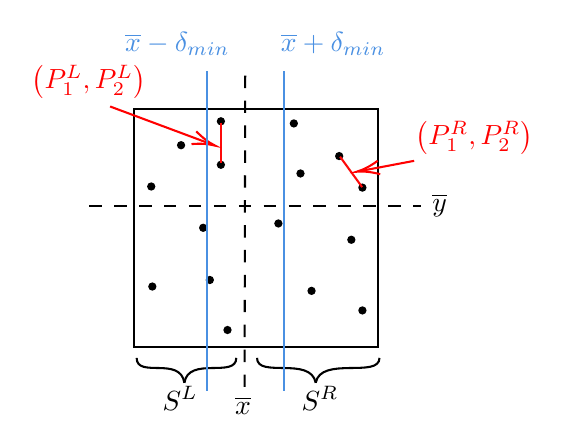
\begin{tikzpicture}[x=0.75pt,y=0.75pt,yscale=-1,xscale=1]
    %uncomment if require: \path (0,325); %set diagram left start at 0, and has height of 325
    
    %Shape: Rectangle [id:dp6499204868826074] 
    \draw   (80.93,157.92) -- (198.12,157.92) -- (198.12,272.62) -- (80.93,272.62) -- cycle ;
    %Straight Lines [id:da837478004805259] 
    \draw [color={rgb, 255:red, 0; green, 0; blue, 0 }  ,draw opacity=1 ] [dash pattern={on 4.5pt off 4.5pt}]  (59.2,204.85) -- (219,204.85) ;
    %Straight Lines [id:da7194776025159269] 
    \draw [color={rgb, 255:red, 0; green, 0; blue, 0 }  ,draw opacity=1 ] [dash pattern={on 4.5pt off 4.5pt}]  (134.31,142) -- (134,295) ;
    %Shape: Free Drawing [id:dp8916770831600931] 
    \draw  [line width=3] [line join = round][line cap = round] (103.41,175.52) .. controls (103.41,175.52) and (103.41,175.52) .. (103.41,175.52) ;
    %Shape: Free Drawing [id:dp7205705113694219] 
    \draw  [line width=3] [line join = round][line cap = round] (179.58,180.76) .. controls (179.58,180.76) and (179.58,180.76) .. (179.58,180.76) ;
    %Shape: Free Drawing [id:dp5723003936317532] 
    \draw  [line width=3] [line join = round][line cap = round] (166.27,245.7) .. controls (166.27,245.7) and (166.27,245.7) .. (166.27,245.7) ;
    %Shape: Free Drawing [id:dp19778776200558257] 
    \draw  [line width=3] [line join = round][line cap = round] (89.56,243.61) .. controls (89.56,243.61) and (89.56,243.61) .. (89.56,243.61) ;
    %Shape: Free Drawing [id:dp22218199289458562] 
    \draw  [line width=3] [line join = round][line cap = round] (150.29,213.23) .. controls (150.29,213.23) and (150.29,213.23) .. (150.29,213.23) ;
    %Shape: Free Drawing [id:dp9270216931653172] 
    \draw  [line width=3] [line join = round][line cap = round] (157.74,165.04) .. controls (157.74,165.04) and (157.74,165.04) .. (157.74,165.04) ;
    %Shape: Free Drawing [id:dp30577755696643694] 
    \draw  [line width=3] [line join = round][line cap = round] (89.03,195.42) .. controls (89.03,195.42) and (89.03,195.42) .. (89.03,195.42) ;
    %Shape: Free Drawing [id:dp8352617777328899] 
    \draw  [line width=3] [line join = round][line cap = round] (125.78,264.56) .. controls (125.78,264.56) and (125.78,264.56) .. (125.78,264.56) ;
    %Shape: Free Drawing [id:dp007121195742592068] 
    \draw  [line width=3] [line join = round][line cap = round] (190.77,255.13) .. controls (190.77,255.13) and (190.77,255.13) .. (190.77,255.13) ;
    %Shape: Free Drawing [id:dp9787419741468635] 
    \draw  [line width=3] [line join = round][line cap = round] (160.94,189.14) .. controls (160.94,189.14) and (160.94,189.14) .. (160.94,189.14) ;
    %Shape: Free Drawing [id:dp05782734388952204] 
    \draw  [line width=3] [line join = round][line cap = round] (114.06,215.32) .. controls (114.06,215.32) and (114.06,215.32) .. (114.06,215.32) ;
    %Shape: Free Drawing [id:dp020809307556031387] 
    \draw  [line width=3] [line join = round][line cap = round] (122.59,184.95) .. controls (122.59,184.95) and (122.59,184.95) .. (122.59,184.95) ;
    %Shape: Free Drawing [id:dp9236450749534464] 
    \draw  [line width=3] [line join = round][line cap = round] (117.26,240.46) .. controls (117.26,240.46) and (117.26,240.46) .. (117.26,240.46) ;
    %Shape: Free Drawing [id:dp9814876804759312] 
    \draw  [line width=3] [line join = round][line cap = round] (185.44,221.08) .. controls (185.44,221.08) and (185.44,221.08) .. (185.44,221.08) ;
    %Shape: Free Drawing [id:dp32677091280799897] 
    \draw  [line width=3] [line join = round][line cap = round] (190.77,195.95) .. controls (190.77,195.95) and (190.77,195.95) .. (190.77,195.95) ;
    %Shape: Free Drawing [id:dp7375869135394859] 
    \draw  [line width=3] [line join = round][line cap = round] (122.59,164) .. controls (122.59,164) and (122.59,164) .. (122.59,164) ;
    %Straight Lines [id:da2008032684012] 
    \draw [color={rgb, 255:red, 253; green, 10; blue, 10 }  ,draw opacity=1 ]   (122.48,164.63) -- (122.48,184) ;
    %Straight Lines [id:da715666979908854] 
    \draw [color={rgb, 255:red, 253; green, 10; blue, 10 }  ,draw opacity=1 ]   (180.01,181.07) -- (190.66,195.74) ;
    %Straight Lines [id:da6970165255401948] 
    \draw [color={rgb, 255:red, 255; green, 0; blue, 0 }  ,draw opacity=1 ]   (215.7,183.06) -- (189.96,187.93) ;
    \draw [shift={(188,188.3)}, rotate = 349.29] [color={rgb, 255:red, 255; green, 0; blue, 0 }  ,draw opacity=1 ][line width=0.75]    (10.93,-3.29) .. controls (6.95,-1.4) and (3.31,-0.3) .. (0,0) .. controls (3.31,0.3) and (6.95,1.4) .. (10.93,3.29)   ;
    %Straight Lines [id:da5840245566165858] 
    \draw [color={rgb, 255:red, 255; green, 0; blue, 0 }  ,draw opacity=1 ]   (69.21,156.87) -- (117.94,175.03) ;
    \draw [shift={(119.82,175.73)}, rotate = 200.44] [color={rgb, 255:red, 255; green, 0; blue, 0 }  ,draw opacity=1 ][line width=0.75]    (10.93,-3.29) .. controls (6.95,-1.4) and (3.31,-0.3) .. (0,0) .. controls (3.31,0.3) and (6.95,1.4) .. (10.93,3.29)   ;
    %Curve Lines [id:da7178341035011966] 
    \draw    (82,278) .. controls (82,288) and (103,277) .. (105,290) ;
    %Curve Lines [id:da31697667567298216] 
    \draw    (130,278) .. controls (130,288) and (107,277) .. (105,290) ;
    %Curve Lines [id:da6058144347191174] 
    \draw    (140,278) .. controls (140,288) and (165.81,277) .. (168.27,290) ;
    %Curve Lines [id:da842179996151678] 
    \draw    (199,278) .. controls (199,288) and (170.73,277) .. (168.27,290) ;
    %Straight Lines [id:da01763770038587964] 
    \draw [color={rgb, 255:red, 74; green, 144; blue, 226 }  ,draw opacity=1 ]   (153,140) -- (153,294) ;
    %Straight Lines [id:da6702110585391772] 
    \draw [color={rgb, 255:red, 74; green, 144; blue, 226 }  ,draw opacity=1 ]   (116,140) -- (116,294) ;
    
    % Text Node
    \draw (223,197.4) node [anchor=north west][inner sep=0.75pt]    {$\overline{y}$};
    % Text Node
    \draw (128,295.4) node [anchor=north west][inner sep=0.75pt]    {$\overline{x}$};
    % Text Node
    \draw (215,162.4) node [anchor=north west][inner sep=0.75pt]  [color={rgb, 255:red, 255; green, 0; blue, 0 }  ,opacity=1 ]  {$\left( P_{1}^{R} ,P_{2}^{R}\right)$};
    % Text Node
    \draw (30,135.4) node [anchor=north west][inner sep=0.75pt]  [color={rgb, 255:red, 255; green, 0; blue, 0 }  ,opacity=1 ]  {$\left( P_{1}^{L} ,P_{2}^{L}\right)$};
    % Text Node
    \draw (93,290.4) node [anchor=north west][inner sep=0.75pt]    {$S^{L}$};
    % Text Node
    \draw (160,290.4) node [anchor=north west][inner sep=0.75pt]    {$S^{R}$};
    % Text Node
    \draw (150,119.4) node [anchor=north west][inner sep=0.75pt]  [color={rgb, 255:red, 74; green, 144; blue, 226 }  ,opacity=1 ]  {$\overline{x} +\delta _{min}$};
    % Text Node
    \draw (75,119.4) node [anchor=north west][inner sep=0.75pt]  [color={rgb, 255:red, 74; green, 144; blue, 226 }  ,opacity=1 ]  {$\overline{x} -\delta _{min}$};
    
    
    \end{tikzpicture}
\end{center}
We now sort all the points in the $T$ by their decreasing $y-$coordinate. Let $T_y$ be the array of points. For each $P_i\in T_y$ define the region $$T_i=\{P_j\in T_y \mid 0\leq y_j-y_i\leq \delta_{min}, j>i\}$$
\begin{center}
	\begin{minipage}{0.7\textwidth}

\begin{lemma}{}{}
	Number of points (other than $P_i$) that lie inside the box is at most 8
\end{lemma}
\begin{proof}
	Suppose there are more than 8 points that lie inside the box apart from $P_i$. The box has a left square part and a right square part. So one of the squares contains at least 5 points. WLOG suppose the left square has at least 5 points. Divide each square into 4 parts by a middle vertical and a middle horizontal line. Now since there are 5 points there is one part which contains 2 points but that is not possible as those two points are in $S_L$ and their distance will be less than $\delta_{min}$ which is not possible. Hence contradiction. Therefore there are at most 8 points inside the box.
\end{proof}\parinn

Hence by the above lemma for each $P_i\in T_y$ there are at most 8 points in $T_i$. So for each $P_j\in T_i$ we find the $d(P_i,P_j)$ and if it is less than $\delta_{min}$ we update the points and the distance
	\end{minipage}
\hspace{1cm}
\begin{minipage}{0.229\textwidth}
	


\tikzset{every picture/.style={line width=0.75pt}} %set default line width to 0.75pt        

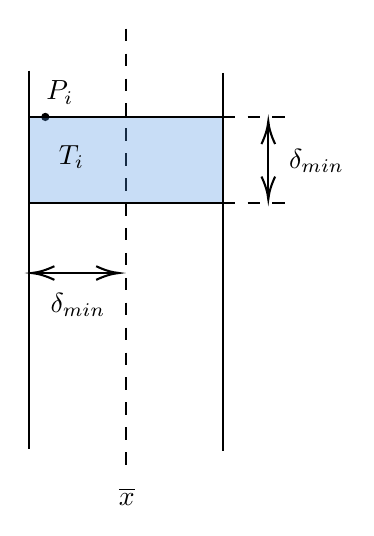
\begin{tikzpicture}[x=0.75pt,y=0.75pt,yscale=-1,xscale=1]
	%uncomment if require: \path (0,300); %set diagram left start at 0, and has height of 300
	
	%Straight Lines [id:da3975720681427135] 
	\draw    (200,50.92) -- (200,233.14) ;
	%Straight Lines [id:da42362227502058447] 
	\draw    (293.43,51.98) -- (293.43,234.2) ;
	%Straight Lines [id:da04130491026490812] 
	\draw  [dash pattern={on 4.5pt off 4.5pt}]  (246.71,30.67) -- (246.71,244.38) ;
	%Straight Lines [id:da4384742510539741] 
	\draw    (200,73.3) -- (293.43,73.3) ;
	%Straight Lines [id:da3745552754160917] 
	\draw    (200,114.85) -- (293.43,114.85) ;
	%Straight Lines [id:da9873374520652576] 
	\draw    (203.43,148.38) -- (241.43,148.38) ;
	\draw [shift={(243.43,148.38)}, rotate = 180] [color={rgb, 255:red, 0; green, 0; blue, 0 }  ][line width=0.75]    (10.93,-3.29) .. controls (6.95,-1.4) and (3.31,-0.3) .. (0,0) .. controls (3.31,0.3) and (6.95,1.4) .. (10.93,3.29)   ;
	\draw [shift={(201.43,148.38)}, rotate = 0] [color={rgb, 255:red, 0; green, 0; blue, 0 }  ][line width=0.75]    (10.93,-3.29) .. controls (6.95,-1.4) and (3.31,-0.3) .. (0,0) .. controls (3.31,0.3) and (6.95,1.4) .. (10.93,3.29)   ;
	%Straight Lines [id:da5826410245797784] 
	\draw    (315.43,77.3) -- (315.43,110.85) ;
	\draw [shift={(315.43,112.85)}, rotate = 270] [color={rgb, 255:red, 0; green, 0; blue, 0 }  ][line width=0.75]    (10.93,-3.29) .. controls (6.95,-1.4) and (3.31,-0.3) .. (0,0) .. controls (3.31,0.3) and (6.95,1.4) .. (10.93,3.29)   ;
	\draw [shift={(315.43,75.3)}, rotate = 90] [color={rgb, 255:red, 0; green, 0; blue, 0 }  ][line width=0.75]    (10.93,-3.29) .. controls (6.95,-1.4) and (3.31,-0.3) .. (0,0) .. controls (3.31,0.3) and (6.95,1.4) .. (10.93,3.29)   ;
	%Straight Lines [id:da8728720299963784] 
	\draw  [dash pattern={on 4.5pt off 4.5pt}]  (293.43,73.3) -- (329.43,73.3) ;
	%Straight Lines [id:da06933695064552192] 
	\draw  [dash pattern={on 4.5pt off 4.5pt}]  (293.43,114.85) -- (324.43,114.85) ;
	%Shape: Free Drawing [id:dp435305414025839] 
	\draw  [line width=3] [line join = round][line cap = round] (208,73.17) .. controls (208,73.17) and (208,73.17) .. (208,73.17) ;
	%Shape: Rectangle [id:dp914080675609527] 
	\draw  [fill={rgb, 255:red, 74; green, 144; blue, 226 }  ,fill opacity=0.3 ] (200,73.3) -- (293.43,73.3) -- (293.43,114.85) -- (200,114.85) -- cycle ;
	
	% Text Node
	\draw (209,156.4) node [anchor=north west][inner sep=0.75pt]    {$\delta _{min}$};
	% Text Node
	\draw (324,87.4) node [anchor=north west][inner sep=0.75pt]    {$\delta _{min}$};
	% Text Node
	\draw (207,54.4) node [anchor=north west][inner sep=0.75pt]    {$P_{i}$};
	% Text Node
	\draw (242,250.4) node [anchor=north west][inner sep=0.75pt]    {$\overline{x}$};
	% Text Node
	\draw (213,85.4) node [anchor=north west][inner sep=0.75pt]    {$T_{i}$};
	
	
\end{tikzpicture}
\end{minipage}
\end{center}
\subsection{Pseudocode and Time Complexity}
\begin{algorithm}
	\DontPrintSemicolon
	\KwIn{Set of $n$ points, $S=\{(x_i,y_i)\mid x_i,y_i\in\bbR, \ \forall\ i\in[n]\}$. We denote $P_i=(x_i,y_i)$. }
	\KwOut{Closest pair of ponts, $(P_i,P_j,\delta)$ where $\delta=d(P_i,P_j)$}
	\Begin{
\If{$|S|\leq 10$}{Solve by Brute Force (Consider every pair of points)}	

$S^x\longleftarrow S$ sorted by $x-$coordinate\;
$S^y\longleftarrow S$ sorted by $y-$coordinate\;
$\bar{x}\longleftarrow \lfloor \frac{n}{2}\rfloor $ highest $x-$coordinate\;
$\bar{y}\longleftarrow \lfloor \frac{n}{2}\rfloor $ highest $y-$coordinate\;
$S^L\longleftarrow \{P_i\mid x_i<\bar{x},\ \forall\ i\in[n]\}$\;
$S^R\longleftarrow \{P_i\mid x_i\geq\bar{x},\ \forall\ i\in[n]\}$\;
$(P_1^L,P_2^L,\delta^L)\longleftarrow$ \textsc{Find-Closest}($S^L$)\;
$(P_1^R,P_2^R,\delta^R)\longleftarrow$ \textsc{Find-Closest}($S^R$)\;
$\delta_{min}\longleftarrow \min\{\delta^L,\delta^R\}$\;
\If{$\delta_{min}<\delta^L$}{$P_1\longleftarrow P_1^R$, $P_2\longleftarrow P_2^R$}

\Else{$P_1\longleftarrow P_1^L$, $P_2\longleftarrow P_2^L$}

}
	\caption{\textsc{Find-Closest}($S$)}	
\end{algorithm}
\chapter{Median Finding}